\chapter{Ideas de la tesis}

\section{Notas para tener en cuenta}

\begin{enumerate}
    \item Lo relacionado con el algoritmo (redes neuronales) y servidor seran los capitulos con mayor densidad de teoria, debido a que no se vio mucho en la carrera.
    \item En la explicación paso a paso se pretende incluir un diagra de bloques del algoritmo, e ir mostrando que hace cada bloque desde un enfoque agnostico al lenguaje, pero recalcando que se utilizo python por su simpleza a la hora de trabajar con redes.
    \item Lo circundante a Docker será mayormente documentación, aunque se explicara la idea y por qué es algo tan utilizado a nivel de industria.
    \item En la implementación fisica de los sensores, se pretende abarcar el montaje, junto con los planos para lograr ensamblar los sensores.
\end{enumerate}

\section{Un repaso rapido por la PIP}

\section{Redes}

\subsection{Introducción a las redes}

Como se comentó uno los ejes de este trabajo se va a basar en la utilización de redes neuronales para la detección y reconocimiento de patentes y sus correspondientes caracteres, entonces ¿Qué es una red neuronal?, a grandes rasgos una red neuronal en un algoritmo computacional que intenta imitar el cerebro humano, en otras palabras es un sistema de computación compuesto por un gran numero de elementos simples que se encuentran interconectados, los cuales procesan la información por medio de estados dinámicos, respondiendo a entradas externas.[acá iría referencia]

Debido a la semenjanza que existe entre los algoritmos de deep learning y el cerebro humano, a la unidad fundamental de estos sistemas se la denomina neurona.
Cada neurona procesa la información de la capa de anterior y la entrega a la siguiente capa. Este proceso se puede entender como la sinapsis neuronal de los seres vivos.
La sinamsis es una suma poderada que puede ser expresada como $Y = W^T\dot X + b$ donde $W$ representa los pesos de la neurona, $b$ es un bias y $X$ es el vector de entrada.

Una capa es un arreglo en paralelo de neuronas, las capas se interconectan para crear redes más complejas capaces de realizar tareas más especificas [agregar figura de una red y sus partes].
Debido a que en esencia el proceso que realiza la neurona es una transformación lineal, al interconectar capas la resultante sigue siendo una transformación lineal. Este problema de linealidad se soluciona apilcando una función de activación luego de la transformación lineal, obteniendo $Y=f(W^T \dot X + b)$. [agregar grafico de funciones de activación].

Para lo que a procesamiento de imagen y extracción de características las redes mas utilizadas son las CNN , ya que su diseño se vaso en la estructura de la corteza visual animal, esta imitación se consigue utilizando la convolución en 2 dimensiones.
La convolución es 2 dimensiones es similar al caso conocido en  1 dimensión con algunas modificaciones, por ejemplo se habla de sistemas LSI (lineales de espacio invariante) en vez de LTI, para tenerla presente se procede a explicar la definición de convolución discreta en 2 dimensiones
Se define filtro o núcleo  o matriz de convolución a la respuesta de un sistema LSI discreto, el filtro es dimensión $2k x 2k$ donde $k$ es un valor establecido arbitrario (usualmente son matrices cuadradas de $3x3$ o $5x5$) que define cuantos valores habra de la muestra.
Se define a $h[n]$ como un filtro de dimension $2k x 2k$ e $I$ una imagen a escala de grises, donde cada punto de coordenadas $(i,j)$ es el resultado de la convolucion entre $h$ e $I$ dado por 
\begin{equation}
O(i,j)= \sum_{u=-k}^{k}n
\end{equation}

HABLAR DE TIPOS DE NEURONAS CONVOLUCIONALES.

FALTA EXPLICAR EL ALGORITMO DE ENTRENAMIENTO MEDIANTE DATASETS Y BACKPROPAGATION.

Existen diversos tipos clasificación aunque la más utilizada es por el rol que la red puede desempeñar, existen redes reunorales convolucionales o CNN por sus siglas en inglés (comúnmente utilizadas para clasificación de imagenes),
reder reuronales recurrenter o RNN (utilizadas para predicción de texto de largo variable), entre otras. Otra clasificación que es posible utilizal es según la cantidad de capas que esta posea, existiendo 2 clasificaciones, simple las cuales no poseen capas ocultas y profundas las cuales si poseen capas ocultas.

A continuación se dará un breve resumen de como se crean estas capas de neuronas, para ello vamos explicar de manera sencilla y concisa como funciona una red neuronal:
\begin{itemize}
    \item Una capa recibe valores, llamados inputs,si se trata de la primera capa esos valores vendrán definidos por los datos de entrada, mientras que el resto de capas recibirán el resultado de la capa anterior.
    \item Luego se realiza una suma ponderada de todos los valores provenientes de la entrada, para ellos se necesita una matriz de pesos llamada W, la matriz tiene filas igual al numero de de capas anterior y columnas igual como neuronas tiene la capa actual.
    \item Al resultado de la suma ponderada se le sumará otro parámetro, conocido como bias o, simplemente, b. Cada neurona tiene su propio bias, por lo que las dimensiones del vector bias depende de la capa, por lo que será una columna y tantas filas como neuronas tiene esa capa.
    \item Luego se requiere de una función de activación, uno de los elementos mas importantes dentro de la red. Ya que hasta ahora solo tenemos una regresión lineal. Para evitar esto, al resultado de la suma anterior se le aplica una función, conocido como función de activación. El resultado de esta función será el resultado de la neurona.
\end{itemize}

Una vez que se realiza la suma ponderada, lo que tenemos es básicamente una transformación lineal, por lo que para evitar esto, se introduce una función que modifica estos datos, conocida como función de activación, que ademas de sacar linealidad a la red, le permite resolver problemas mas complejos, algunas de las mas usadas son la funcion escalon, la funcion sigmoide, la funcion rectificadora ReLU y la funcion tangete hiperbolica.[poner graficos]


vamos a hablar sobre redes neuronales basadas en imágenes (CNN) y sobre yolo v4.

nuestro algoritmo de entrada/salida \\

explicar como van a funcionar los sensores SL y SL mini a nivel de control de entrada salida,
como lo vamos a hacer, es decir hablar de las 2 redes que vamos a usar. \\



explicación del algoritmo paso a paso \\

se pretende explicar como funciona la cada parte de nuestro algoritmo, y que hace cada una de las redes, mostrando que la red que reconoce los caracteres no lo hace de forma consistente si la imagen no es recortada previamente. Hablamos sobre la yolo v4 y sus ventajas junto con su arquitectura.



\section{Server}

En este apartado se busca hablar sobre el servidor, su arquitectura basada en microservicios usando docker, y la base de datos.

\subsection{Un viaje rapido por el servidor}

El servidor posee una arquitectura de microservicios Fig \ref{fig:server}, donde todos los servicios corren en Docker. Las barreras interactuan hacia el servicio de NestJS donde se suben los registros de entrada/salida, para luego procesar las imagenes (Solo en el caso del SL mini) mediante el servicio de Flask, para obtener la patente como texto. Los clientes pueden acceder a Grafana para visualizar datos tales como (DAR EJEMPLOS CUANDO ESTEN). La base de datos se mantiene aislada del exterior, por lo que no es posible acceder a ella directamente, y solo se puede interactuar mediante el servicio de NestJS.

\begin{figure}
        \centering
        
\includegraphics[width=.5\textwidth]{imgs/uncoma.png}
        \caption{Arquicetura del servidor}
        \label{fig:server}
\end{figure}

\subsection{Docker}

Docker es una plataforma de software que permite crear, probar e implementar aplicaciones mediante el uso de contenedores.

\subsubsection*{Contenedores}


Un contenedor de Docker funciona como una maquina virtual, practicamente aislada del sistema. La gran diferencia entre un contenedor y una maquina virtual es que el contenedor solo realiza una virtualización de capas por encima del sistema operativo, por lo que el contenedor comparte el kernel con el sistema padre, mientras que la maquina virtual emula todo incluido el kernel del sistema, esto produce que los contenedores sean más eficientes en el uso del hardware, pero altamente dependientes del kernel del sistema padre. Es por ello que un SO Windows no puede correr contenedores Linux de una forma sencilla y debe recurrir a una virtualización del kernel Linux Fig. \ref{fig:docker-funcinamiento}.


\begin{figure}
        \centering
        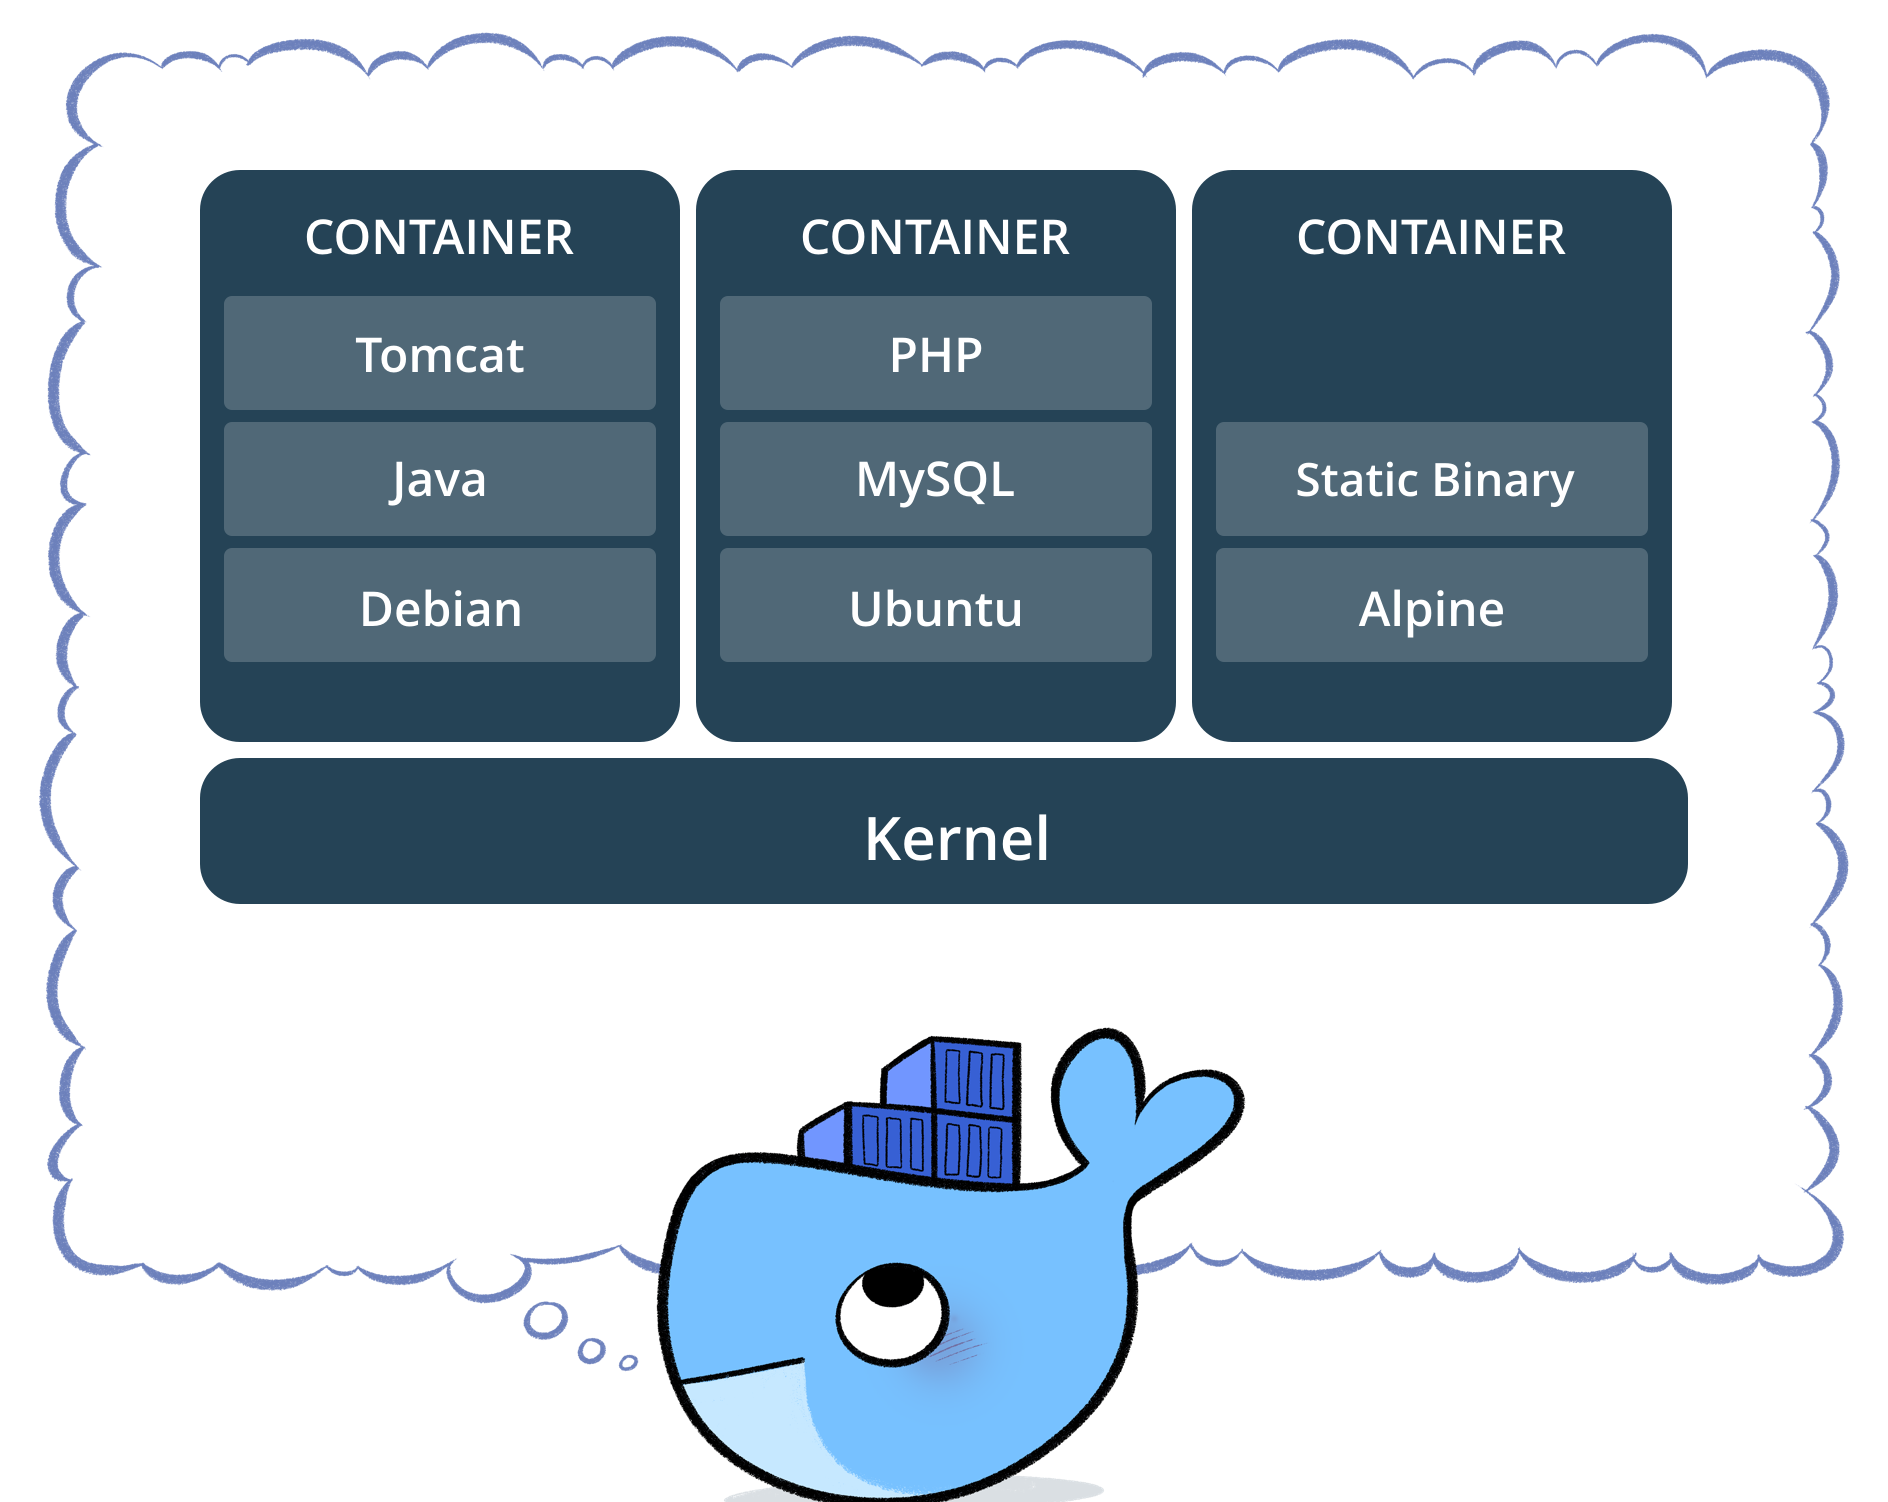
\includegraphics[width=.5\textwidth]{imgs/contenedores-docker.png}
        \caption{Funcionamiento de Docker}
        \label{fig:docker-funcinamiento}

\end{figure}

Una pregunta frecuente es: como guardo información que tengo en mi contenedor de docker en mi maquina? la solución a esta pregunta son los volumenes los cuales son un puente entre una carpeta de nuestra pc y una carpeta del contenedor, esto nos permite que cualquier archivo que contenga la carpeta de nuestra PC se encuentre en el contenedor, y viceversa. Esta comunicacíon entre el contenedor y nuestra PC nos permite realizar varias tareas, como realizar backups de la base de datos, compartir archivos de configuración para los diferente servicios.

\subsection{Docker compose}

A la hora de manejar varios contenedores el uso del interfaz de linea de comandos o CLI (por sus siglas en inglés) de Docker se vuelve engorrozo, es por ello que existen varios sistemas que tratan de simplificar y automatizar la tarea de levantar contenedores o servicios como los llamaremos de aquí en adelante. Una de estas tecnologías es Docker compose la cual permite definir dentro de un archivo yaml la arquitectura de los diferentes servicios [https://docs.docker.com/compose/], junto los volumenes y redes internas.

Cabe destacar que Docker compose crea una red interna en la cual (salvo que definamos de otra manera) todos los contenedores estan interconectados y podemos relacionarnos usando el nombre del servicio como url.

\subsection{Frontend vs Backend}

comparacion de los servicios frontend y backend explicando sus diferencias


\subsection{Microservicios}

La arquitectura de microservicios es una unión de servicios autónomos y pequeños. Esto nos permite que cada servicio utilice una tecnología diferente, siempre que sea necesario. En este trabajo se utiliza un servicio principal que utiliza NestJS (Javascript) y otro que utiliza Flask (Python), ya que Python posee una gran cantidad de herramienta para analisis de datos, mientras que Javascript junto con NestJS permite el desarrollo de un Backend mucho más confiable y rapido. Cada uno de estos servicios corre sobre un contenedor Docker indivual.

El servidor cuenta con los siguientes microservicios:

\begin{enumerate}
        \item Base de datos
        \item Applicacion backend con nestjs
              \subitem Usuarios
              \subitem Barreras
              \subitem Parques de estacionamiento
              \subitem Registros
        \item Frontend con ReactJS
        \item Applicacion backend con Flask (analisis de patente online)
        \item [no implementada] Grafana para usuarios
\end{enumerate}


\subsection{Backend con NestJS}


Para la autenticación se utilizo el module de Passport JS, el cual permite crear estrategias para los diferentes tipos de autenticación, las estrategias utilizadas son:

\begin{enumerate}
        \item Local
        \item Apikey aplicaciones de terceros
        \item Apikey para las barreras
        \item JWT
\end{enumerate}

La estrategia Local, hace un logging del usuario segun su nombre de usuario y su contraseña.

Los servicios de apikey buscan que la apikey sea valida, es decir, se encuentre en la base de datos vinculada a una barrera, o este dentro de las apikeys validas de aplicaciones, en este caso solo 2 servicios se encuentran habilitados para realizar peticiones (Frontend y Grafana)

Un JSON Web Token es un estandar qué esta dentro del documento RFC 7519, este define un mecanismo para enviar información entre 2 partes, en este caso cliente-servidor de forma segura (utilizando cifrado). Los datos son codificados en un objeto de javascript (JSON),

\subsection{El cerebro de la aplicación}

Si bien, las barreras procesan datos antes de enviarlos, la logica del sistema se encuentra implementada en el server, corriendo bajo el servicio de NestJS, es decir el backend de nuestra app. Este servicio se encarga de interconectar la base de datos con lo requerido por los clientes, y las barreas. La idea es describir como maneja las peticiones mas importantes, que serian desde grafana, desde una app externa (como la pagina donde el usuario pide las barreras), y las peticiones de la misma barrera, siendo esta un apartado meramente tecnico de detalles de implementacion.


\subsection{Frontend con ReactJS}

Basicamente se va a hablar del panel admin y algun funciones para los clientes. junto con las librerias implementadas como ZOD,

\begin{enumerate}
        \item Manejo de estado global: https://docs.pmnd.rs/zustand/getting-started/comparison
        \item ZOD: https://zod.dev/
\end{enumerate}

Existen 2 clientes frontend uno para la adminitracion y otro para los clientes.

\subsubsection{Clientes}

La web para los clientes tienen una pagina de autenticación (ver figura), en esta web los clientes pueden darse de alta y entrar a su session, el manejo de la session se hace atravez de json web token, como fue nombrado en el apartado de backend.

En esta web los clientes pueden a los lugares que tiene a cargo, ya que se permite más de un lugar por usuario. Si el cliente posee lugares puede acceder a la tienda para encargar barreras, como minimo un lugar debe poseer 2 barreras.

Ademas los clientes pueden configurar las barreras de manera atravez de la plataforma web, los parametros de configuración [deben haber sido nombrados en la sección del algoritmo de la barrera]. 

\subsection{Grafana}

Hablar sobre los dashboard

\subsection{Mqtt broker}

hablar sobre el protocolo, sus utilidades y para que se usa en el sistema. Su funcion principal es que la barrera avise al servidor cada X tiempo que esta activa,
esto sirva para en el futuro implementar sistemas de aviso cuando una barrera deberia estar prendida y no lo esta o viceversa. Ademas se utiliza para enviar las configuraciones de la misma ante algun cambio que el usuario desee.


\subsection{Base de datos}

explicacion de base de datos relacional y no relacional, por qué elegimos mongoDB para el almacenamiento de datos. Y qué es lo que se guarda. Tambien se explicara como se guardan las imagenes. \\




\section{Montaje Real}

Se pretende mostrar como esta montado el sensor, hablar sobre las decisiones de diseño, tanto
camara, como alimentación. Tambien se pretende incluir un analisis de consumo. y resultados de las pruebas, mostrando tanto datos, como imagenes de los resultados. En este apartado la teoria se basara mas que nada en alimentacion y detalles sombre las camaras. \\




\section{Pruebas}
Para la correcta verificación del funcionamiento de ambos conjuntos de software y hardware se planificaron una serie de pruebas que pongan a corroboren que el diseño cumple su labor de manera optima.
Por lo que luego de analizar que parámetros son los que mas influyen a la hora de la colocación del pack sensor-cámara, se llego a la conclusión de que los parámetros que mas influyen son 3, distancia entre vehículo y la cámara, angulo de la cámara y la intensidad de luz necesaria para que el algoritmo reconozca las patentes.

\subsection{Prueba de ángulos y distancia}
Para esta prueba se busco obtener la distancia y angulo optima para que el algoritmo pueda obtener la patente sin perjudicar el acceso al estacionamiento, la misma se realizara en un mismo día, en el que las condiciones climáticas sea lo mas optimas posibles para no perjudicar la prueba.
La primer parte de la prueba consta de obtener una imagen desde el mismo angulo aumentando la distancia en intervalos regulares, comenzando por $poner distancia minima$ para luego ir aumentando en $poner distancia$, hasta el punto que el algoritmo no sea capaz de obtener los caracteres de la patente.
Los resultados se pueden observar en la tabla (acá va la referencia la tabla) junto con los caracteres obtenidos.
Con la primer parte concluida y los resultados obtenidos se toma el valor considerado mas optimo para manterlo fijo e ir cambiando la posición de la cámara sobre una circunferencia para modificar el angulo respecto a la patente.
Como el resultado de angulo $0$ ya se tiene se ira realizando un barrido en angulo equiespaciado a razon de $poner cantidad$ hasta llegar a que el angulo sea $90$.


\subsection{Pruebas a diferente luz}

Todavia falta evaluar como se realizara esta prueba, pero la idea es probar como procesa la red fotografias con luz natural, de noche, y con luz artificial.

\subsection{Un estacionamiento real}

La idea seria, ir al estacionamiento de la facu, finde semana y probar cuanto tarda la red en reconocer las patentes.

\subsection{Conclusión}

Conclusiones del capitulo, analisis de la viabilidad del proyecto en entornos reales. Propuestas de posibles mejoras o nuevas funcionalidades que permitan su uso en otras tareas, una idea a día de hoy, es implementar un filtro de patentes por lugar, para solo permitir que accedan algunos vehiculos, como pasa en parques de estacionamiento de empresas.


